\pagebreak

\chapter{Overview}

    3PL is a language intended to allow parallel algorithms to be coded for
    implementation in an FPGA. A language which compiled directly into an FPGA
    configuration was considered insufficient on its own since it is often necessary
    to run an algorithm which in turn generates the target algorithm. For example an
    extreme case is a batcher sorting network where the batcher algorithm must be
    executed to generate the network topology. In simpler cases it is an advantage
    to parameterise the target algorithm which again implies some sort of
    preliminary processing. This could be accomplished by using a general purpose
    language such as C, Java or Python to pre-process the target algorithm, but it
    was decided that it was preferable to combine all of this in one language. Thus
    3PL is actually a sequential language similar in most respects to C, but it has
    additional statement types that generate FPGA target code. This might have been
    accomplished by adding appropriate classes to Java or Python but it was felt
    that a new language tailored to the task would be preferable.    
    
    3PL was designed to meet several criteria -
    
    \blist
    \item   it must provide constructs within the FPGA such as variables, memory
    and combinatorial logic.
    \item   it must provide execution threads which include
    sequential operations, parallel operations and looping and conditional control.
    \item   it should provide a mechanism whereby systolic pipelines can be
    constructed which are data driven.
    \item   the control of execution threads must co-exist with data-driven
    execution.
    \item   it should be concise.
    \blend

    3PL is really two languages in one. 3PL is compiled and then executed
    by an interpreter. That execution, called {\em immediate} execution,
    \index{immediate execution}
    is strictly sequential. During immediate execution target (FPGA)
    statements are encountered. These target statements are also subject
    to immediate execution during which target code is generated which
    will later be executed in the FPGA. For example the code
    \begin{lstlisting}[gobble=4, language=threepl]
       par {
           a <- b;
           c <- d;
       }
    \end{lstlisting}
    looks like a parallel block in which two assignments execute
    simultaneously. While that is exactly what it ultimately represents the
    way 3PL handles this is a little more complicated. The {\em par}
    construct and the assignments are subject to immediate execution -
    first the {\em par} and then each of the nested assignment statements
    in turn. Immediate execution of the {\em par} creates a parallel block
    structure in the target code and then each nested statement in the
    block is executed in turn. If immediate execution of a nested statement
    generates in-line target code then that code is linked into the
    parallel block that has been created for subsequent parallel execution
    in the target. In the example each assignment statement generates
    in-line target code and that target code will be linked into the
    parallel block.

    This description may seem pedantic, but once immediate and target
    statements are intermixed it becomes important to understand the way
    3PL executes. As a more complicated example consider the following -
    \pagebreak
    \begin{lstlisting}[gobble=4, language=threepl]
       par {
           for(int(i) ; i<10 ; i=i+2)
               a[i] <- b[i];
       }
    \end{lstlisting}
    In this example we can again follow the previous description to see
    what is generated. Immediate execution of the {\bf par} creates a
    parallel block for the target. Immediate execution of the nested {\bf
    for} does not itself create target code, but the immediate
    execution of the code within the loop creates a target assignment
    statement on each iteration. Immediate execution of each target
    assignment statement generates in-line target code which is passed
    back to the enclosing {\bf par}. In this case the 5 iterations produce
    5 target assignments which are handled by the enclosing {\bf par}. The
    generated target code is equivalent to having written -
    \begin{lstlisting}[gobble=4, language=threepl]
       par {
           a[0] <- b[0];
           a[2] <- b[2];
           a[4] <- b[4];
           a[6] <- b[6];
           a[8] <- b[8];
       }
    \end{lstlisting}
    
    Note that this oversimplified example is contrived - it could have
    been coded as
    
    \begin{lstlisting}[gobble=4, language=threepl]
        a <- b;
    \end{lstlisting}

    The {\bf 3PL} language contains two distinct types of statements -
    \blist
    \item    {\em immediate} statements
    \item    {\em target} statements
    \blend

    Immediate statements \index{immediate!statement} are executed by the
    compiler in the host computer following parsing. They control the processing
    of target statements.

    Target statements \index{target!statement} are to be executed in the FPGA
    later - they perform the actual data processing.

    The {\bf 3PL} compiler parses the source code and stores a
    representation of the code internally.

    The compiler then executes the entire {\bf 3PL} program sequentially.
    Immediate statements are explicitly executed. Target statements when
    encountered generate logic elements into a target code structure.
    Module, procedure and function calls are executed by the interpreter but
    any target code they generate is produced for each instance.
    Immediate variables occurring in target code are replaced by their
    current value.

    Immediate and target statements are distinguished by the compiler by
    their different syntax. This was a design decision intended to make
    the code more readable - immediate and target constructs are easily
    distinguished by inspection. The alternative would be to use the same
    syntax for immediate and target code and distinguish them by the mode
    of variables - easily implemented but resulting in more difficulty in
    reading and maintaining 3PL code.

    The philosophy of \Index{queue} variables is that pipelines
    \index{pipeline} of processing modules can be simply strung together
    using queue variables to convey data from one to the next. Where this
    differs from the usual sort of readable/writable channel is that -
    \blist
    \item   queue variables can go to multiple destinations, all of which
            must read before the source will make the next datum available
    \item   queue reads and writes occur in the source code as normal
            variable value references and assignments, not explicit read
            and write statements
    \blend
    Such a pipeline does not necessarily advance on every clock cycle,
    but rather modules process data in their own time when it is
    available, then pass it on. This mechanism does not incur any speed
    penalty as a pipeline can run at the full clock rate unless a module
    takes more than one cycle because of the nature of the algorithm.

    In addition to the dataflow mechanism provided by queue variables 3PL
    fully supports simple register variables and execution control
    constructs such as sequential and parallel blocks, loops and
    conditionals. 3PL also provides a simple implementation of Petrinets which
    are more general than state machines. Queues and other variable modes can
    be compound types such as arrays or structs. These can be nested, and
    array members or struct fields can be accessed in parallel. Target array
    members can also be selected using variable subscripts.

    Hardware elements explicitly implemented include 3-state buses,
    priority encoders, combinatorial output multiport RAMs (Xilinx single
    or dual port CLB distributed RAM) and registered output multiport
    RAMs (Xilinx single or dual port block RAM).

    Low level optimisation at the netlist level explicitly for Xilinx
    includes use of the carry chain for wide logic gates, decoders and
    priority encoders, and CLB shift registers for some delay functions.

    3PL supports any number of clocks and provides a means of
    resynchronising data between clock domains.

    Intermediate code allows the use of pointers (both to immediate and
    to target variables) so that linked data structures can be
    constructed. Variables are created during immediate execution
    (interpretation) and continue to exist after their scopes have
    vanished, neatly solving the allocation problem (thus a function can
    return a pointer to a local variable which can continue to be used
    via the pointer after the function returns).


    
    

    \section{Variable modes}

        Variables in 3PL fall into 11 categories, referred to as {\bf modes}. These are -

        \kwd{Immediate} - an immediate variable only exists during execution of the 3PL interpreter.
        When a 3PL program is executed by the interpreter immediate mode variables are
        used in the same way as variables in languages such as C. Immediate mode variables
        do not generate FPGA code and are not represented in the FPGA configuration in any way.
        Immediate mode variables can be integer, boolean, floating point, string, array,
        struct, pointer, file or enumerated types. Immediate execution is discussed later.

        A program containing only immediate mode variables will execute in a similar way to
        a C program and no FPGA code will be involved.

        The remaining modes are all 'target' modes, that is they represent hardware devices
        in the FPGA.

        \kwd{Static} - a static variable is a register in the FPGA. It can be integer, unsigned
        integer, fixed point, unsigned fixed point, floating point, boolean, array or struct
        types. All except the boolean type must have bit widths specified.

        \kwd{Queue} - a variable which is a queue. If it is evaluated in a statement a datum
        will be popped. If it is assigned, a datum will be pushed. Otherwise it appears in
        statements and expressions in the same way as other variables. In any context a
        statement using a queue variable will wait to execute if the variable is not
        'available', i.e. has a datum to pop or a free space in which to push a datum as
        appropriate.

        \kwd{Value} - a value variable can represent any expression. The expression could be
        as simple as a single static or queue variable, in which case the value variable is a bit
        like a pointer.

        \kwd{Selectvalue} - a variable which can select one of many inputs dynamically. In earlier
        FPGAs this would be implemented by 3-state buffers, but in later platforms the
        implementation uses combinatorial logic. These variables are used to construct buses
        internal to the FPGA.

        \kwd{Priority} - a priority variable implements a priority encoder. It is combinatorial
        logic which appears as a boolean array where multiple simultaneous inputs are blocked
        except for that with the highest priority.

        \kwd{Input} - these provide an interface for input pads.

        \kwd{Output} - output variables drive 2-state or 3-state output pads.

        \kwd{Clock} - clock variables provide clocks for the synchronous logic which 3PL produces.
        Connections between clock inputs, clock managers and clock buffers are also clock mode
        variables.

        \kwd{Rmemory} - these create registered-output memory, implemented at the moment by
        block RAM.

        \kwd{Cmemory} - these create combinatorial memory, implemented using CLB RAM.




    \section{Static mode variables}

        The most straightforward of the target modes is \kwd{static}. A static mode variable
        is equivalent to a normal variable in programming languages such as C or
        Java. It is implemented in the FPGA as a register using flip-flops. A static
        variable stores a value and therefore has state.

        The following code shows the creation of a static variable and an assignment
        to it -
        \begin{lstlisting}[language=threepl]
            static(v, "int:8");
            v <- 3;
        \end{lstlisting}
        The string "int:8" gives the type of the variable, which is an 8-bit integer.

        The assignment operator for a static variable is \verb'<-'. There are a number
        of different assignment operators for different variable modes, the intention
        being to make the modes immediately distinguishable on inspection of source
        code without the need in most cases to look for the statement creating
        the variable. Thus an assignment using \verb'<-' immediately indicates that
        the variable on the left side is a static variable.

        The assignment takes one clock cycle.

        On assignment the widths of the left and right hand sides of the assignment
        need not be the same, however in that case padding or truncation will result.
        If the type is signed then padding will be by sign extension, otherwise
        zero padding is used.

        3PL has the unusual characteristic that FPGA statements execute repeatedly,
        i.e. as if they were enclosed in infinite loops. The reason for this design
        decision is that FPGA statements are intended to operate on data streams
        and to do so with a high degree of parallelism. Thus every statement can
        potentially execute on every clock cycle and it is up to conditional
        code to control when statements execute. In a parallel data-driven
        system it seems more sensible to have execution on every clock cycle as
        the default with an overriding conditional mechanism to choose when to execute,
        rather than to enclose every statement in an explicit iteration loop.

        In the example above the variable \var{v} will be assigned 3 on every clock
        cycle. This is not very useful, so we could use a conditional statement
        to exercise some control, e.g. 
        \begin{lstlisting}[language=threepl]
            static(v, "int:8");
            static(l, "log");
            when (l)
                v <- 3;
        \end{lstlisting}
        Here we have introduced another static variable \var{l} which has a logical
        (boolean) type. When \var{l} is true, \var{v} is assigned 3. Now the
        \kwd{when} is executed repeatedly and if \var{l} is true the assignment is
        executed otherwise (since there is no \kwd{else} block) nothing is executed.
        Note that the \kwd{when} does not wait for \var{l} to be true, it simply
        evaluates \var{l} on every one of its continuous iterations and when
        true executes the code body, in this case a single assignment. To make the
        example more useful we could implement a controlled counter by the code -
        \begin{lstlisting}[language=threepl]
            static(v, "int:8");
            static(l, "log");
            when (l)
                v <- v + 1;
        \end{lstlisting}
        where \var{v} is incremented on clock cycles when \var{l} is true. 3PL
        allows the special case of addition or subtraction of one to/from a variable
        to be written using \verb'++' and \verb'--' unary operators, e.g.
        \begin{lstlisting}[language=threepl]
            static(v, "int:8");
            static(l, "log");
            when (l)
                v++;
        \end{lstlisting}
        but note that these operators cannot be used on a static variable as part
        of an expression. We could make the counter bi-directional, e.g.
        \begin{lstlisting}[language=threepl]
            static(v, "int:8");
            static({l, up}, "log");
            when (l)
                when (up)
                    v++;
                else
                    v--;
        \end{lstlisting}
        where when \var{l} is true \var{v} will be incremented if \var{up} is true
        or decremented if \var{up} is false. As illustrated here many variable
        creation procedures allow lists of variables in braces where more than
        one variable of the same type is required.

        The above example is quite correct, however it is preferable to avoid
        nested conditional statements where possible as this can lead to long
        path delays in the FPGA logic. We could recode the example as follows -
        \begin{lstlisting}[language=threepl]
            static(v, "int:8");
            static({l, up}, "log");
            when (l && up)
                v++;
            when (l && !up)
                v--;
        \end{lstlisting}
        which achieves the same behaviour but reduces logic depth at the expense
        of logic width. It could also be written as -
        \begin{lstlisting}[language=threepl]
            static(v, "int:8");
            static({l, up}, "log");
            when (l)
                v <- up ? v+1 : v-1;
        \end{lstlisting}
        using the \verb'?:' ternary operator.

        Static variables have default initial values which are 0 for numeric types
        and false for the logical type. A static variable can be given an initial
        value by means of the optional 3rd argument to procedure \var{static()},
        e.g.
        \begin{lstlisting}[language=threepl]
            static(v, "int:8", 117);
        \end{lstlisting}
        will give static variable \var{v} an initial value of 117. If numeric the
        initial value can of course use hexadecimal (0x...), octal(0...) or binary
        (0b...) notation.
 
    \section{Input and output mode variables}

        We need to be able to get data into and out of the FPGA. For this purpose
        there are two variable modes, \kwd{input} and \kwd{output}.

        An input mode variable represents signals coming into the FPGA via
        pads and input buffers. The following code latches input data into
        a static variable when an enable signal is high -
        \begin{lstlisting}[language=threepl]
            str(enable_pin, "D8");
            var(din_pins, "[8]str", {"A1", "A2", "B1", "B2", "C1", "C2", "D1", "D2"});
            input(d_in, "int:8", loc=din_pins);
            input(enable, "log", loc=enable_pin);
            static(d, type(d_in));
            when (enable)
                d <- d_in;
        \end{lstlisting}
        Input mode variables are created by calling input() which has three or more
        arguments.

        The first argument to input() is an identifier for the created variable.

        The second argument to input() is the type, in this case one is an integer
        of 8 bits and the other is logical (boolean) and hence is implicitly one bit.

        The third and following arguments are attributes for the input. This can
        include FPGA pins (required), a timing group identifier string, a flag
        to control the inserted input path delay, a flag to indicate that an IBUFG
        is to be used rather than an IBUF and finally flags for pullups or pulldowns.
        The attributes are passed in the form attribute=value.

        In general arguments can be passed by position in the normal way or else by
        key=value where key is the name of the parameter for which the argument is
        intended (this is referred to in the 3PL manual as keymatch format). Keymatch
        format is useful where the parameters are many and the arguments are sparse.
        In 3PL arguments are optional and parameters can have default values specified
        for cases where no argument is passed to them.

        In the code above the \var{loc} attribute must either be a string (for a
        single pad) or an array of strings. These are used to generate FPGA pad
        location constraints. Note that array dimensions precede the array type.

        A string immediate mode variable can be created by calling \kwd{str()}.
        The first argument is an identifier for the variable or else a list of
        identifiers in brackets. The second argument is optional and is the initial
        value of the string.

        An array of strings is created by the \kwd{var()} procedure. This is the basic
        variable creation procedure for most modes of variable, procedures such
        as \kwd{static()}, being convenient equivalents. The code
        \begin{lstlisting}[language=threepl]
            static(l, "log");
            str(s, "a_string");
        \end{lstlisting}
        is equivalent to
        \begin{lstlisting}[language=threepl]
            var(l, static, "log");
            var(s, "str", "a_string");
        \end{lstlisting}
        If the second argument is not a mode identifier then it is interpreted as the
        variable type and the mode is assumed to be immediate. The var() procedure entry in
        the 3PL manual should be consulted for more details.   

        The input mode example above assigns the input mode variable \var{d\_in} to
        the static variable \var{d} when the input mode variable \var{enable} is true
        (high).

        Note the use of the function {\bf type()} in the example - this simply returns the
        type of its argument, providing a simple way of creating a variable whose type
        is the same as another.

        The above example would produce a fatal error in 3PL as the input variable {\var
        enable} is used to control conditional logic but is driven by an external
        source and has no timing information with respect to the current clock, so
        there could potentially be timing violations. The usual way to handle this
        is to register the inputs. We can also instruct the place-and-route
        software to place the register flip-flops in an I/O block by setting
        an attribute -

        \begin{lstlisting}[language=threepl]
            str(enable_pin, "D8");
            var(din_pins, "[8]str", {"A1", "A2", "B1", "B2", "C1", "C2", "D1", "D2"});
            input(d_in, "int:8", loc=din_pins);
            input(enable_in, "log", loc=enable_pin);
            static(d, type(d_in), IOB=true);    // locate flip-flops in IOB blocks
            static(enable, "log", IOB=true);

            static(dd, type(d));

            d <- d_in;
            enable <- enable_in;

            when (enable)
                dd <- d;
        \end{lstlisting}
        With the inputs d\_in and enable\_in now latched into flip-flops within I/O blocks
        we minimise the delay between input pad and flip-flop D pins. The clock used for
        this logic must bear an appropriate phase relationship with the external data input
        such that setup and hold constraints are met.

        We could expand the example by connecting the static variable {\var{dd}} to output
        pins -
        \begin{lstlisting}[language=threepl]
            str(enable_pin, "D8");
            var(din_pins, "[8]str", {"A1", "A2", "B1", "B2", "C1", "C2", "D1", "D2"});
            var(dout_pins, "[8]str", {"E1", "E2", "F1", "F2", "G1", "G2", "H1", "H2"});
            input(d_in, "int:8", loc=din_pins);
            input(enable_in, "log", loc=enable_pin);
            static(d, type(d_in), IOB=true);
            static(enable, "log", IOB=true);
            output(,, dd, loc=dout_pins);

            static(dd, type(d));

            d <- d_in;
            enable <- enable_in;

            when (enable)
                dd <- d;
        \end{lstlisting}

        The output() procedure has four or more arguments. The first is an identifier,
        but since in this case we have no need to refer to it we need no identifier so
        the argument is omitted. The second argument is the type, but the type can be
        inferred from the third argument so again the argument can be omitted. The
        third argument is optional and is the source to be used for the output (there
        are other ways of connecting an output mode variable to its source, in which
        case the third argument would be omitted but the first two would be required).
        The fourth and following arguments provide attributes as for the input()
        procedure. In this case they can include slew rate and drive current, the pin
        locations again being mandatory.

        The \var{output()} statement connects the static variable {\bf out} to the FPGA
        pads using output buffers. This example could be re-written to make the
        output assignment explicit -

        \begin{lstlisting}[language=threepl]
            str(enable_pin, "D8");
            var(din_pins, "[8]str", {"A1", "A2", "B1", "B2", "C1", "C2", "D1", "D2"});
            var(dout_pins, "[8]str", {"E1", "E2", "F1", "F2", "G1", "G2", "H1", "H2"});
            input(d_in, "int:8", loc=din_pins);
            input(enable_in, "log", loc=enable_pin);
            static(d, type(d_in), IOB=true);
            static(enable, "log", IOB=true);       
            static(dd, type(d));
            output(out, type(dd),, loc=dout_pins);

            d <- d_in;
            enable <- enable_in;

            when (enable)
                dd <- d;

            out := dd;
        \end{lstlisting}

        note that the last assignment is immediate, not target. It is like assignment
        to a value variable and hence uses the same assignment operator. It is
        an unconditional assignment, i.e. it is connected continuously and not
        changed dynamically. It connects
        the value on the RHS to the output buffers described by the output mode
        variable on the LHS.

        If we want to drive a three-state output pad one cycle after the assignment
        to \var{d} we need conditional output mode assignment. The code might be -

        \begin{lstlisting}[language=threepl]
            str(enable_pin, "D8");
            var(din_pins, "[8]str", {"A1", "A2", "B1", "B2", "C1", "C2", "D1", "D2"});
            var(dout_pins, "[8]str", {"E1", "E2", "F1", "F2", "G1", "G2", "H1", "H2"});
            input(d_in, "int:8", loc=din_pins);
            input(enable_in, "log", loc=enable_pin);
            static(d, type(d_in), IOB=true);
            static(enable, "log", IOB=true);       
            static(enable_del, "log");
            static(dd, type(d));
            output(out, type(dd),, loc=dout_pins);

            d <- d_in;
            enable <- enable_in;
            enable_del <- enable;

            when (enable)
                dd <- d;

            when (enable_del)
                out |- dd;
        \end{lstlisting}

        where the last statement is a conditional target assignment, i.e. a
        three-state assignment. There is a library function \var{delayline()} which
        we could use instead of the assignment to an extra variable -

        \begin{lstlisting}[language=threepl]
            str(enable_pin, "D8");
            var(din_pins, "[8]str", {"A1", "A2", "B1", "B2", "C1", "C2", "D1", "D2"});
            var(dout_pins, "[8]str", {"E1", "E2", "F1", "F2", "G1", "G2", "H1", "H2"});
            input(d_in, "int:8", loc=din_pins);
            input(enable_in, "log", loc=enable_pin);
            static(d, type(d_in), IOB=true);
            static(enable, "log", IOB=true);       
            static(dd, type(d));
            output(out, type(dd),, loc=dout_pins);

            d <- d_in;
            enable <- enable_in;

            when (enable)
                dd <- d;

            when (delayline(enable, 1))
                out |- dd;
        \end{lstlisting}



    \section{Value mode variables}

       Consider the following code fragment -
        \begin{lstlisting}[language=threepl]
            static({a, b, c, d, e}, "int:8");
            a <- c + d + e;
            b <- c + d - e;
        \end{lstlisting}
        This creates five static variables, \var{a}, \var{b}, \var{c}, \var{d}
        and \var{e}, each of
        type "int:8", i.e. an 8-bit integer.
        The second statement assigns an expression containing \var{c}, \var{d}
        and \var{e} to \var{a} on every clock cycle. Similarly the third statement
        also assigns an expression to \var{b}. In each case expressions will be
        implemented by adders and subtracters but the 3PL compiler will not recognise
        the common sub-expression $c + d$. It is a waste of limited logic resources
        to duplicate the sub-expression so we need a way to extract the common
        sub-expression. A \kwd{value} mode variable provides the means to do this.
        \begin{lstlisting}[language=threepl]
            static({a, b, c, d, e}, "int:8");
            value(v, "int:8");
            v := c + d;
            a <- v + e;
            b <- v - e;
        \end{lstlisting}
        Here the value variable represents the expression $c + d$ which is thus
        only instantiated once, the output being shared by the two static assignments.
        The assignment operator for a value mode variable is \verb':='.
        The assignment could be avoided by using the optional initialiser argument
        to the value() procedure -
        \begin{lstlisting}[language=threepl]
            static({a, b, c, d, e}, "int:8");
            value(v, "int:8", c + d);
            a <- v + e;
            b <- v - e;
        \end{lstlisting}

        A value variable thus does not itself have state, i.e. there is no memory
        associated with a value variable. Note the following however -
        \begin{lstlisting}[language=threepl]
            static({a, b}, "int:8");
            value(v, "int:8", b);
            a <- v;
        \end{lstlisting}
        Here the value variable has as its value a single static variable. In this
        role it can be viewed as a pointer to that static variable (3PL does have
        pointer variables).

        Value variables can be re-assigned at any time at which point they take on a
        new value. Value variables can also be evaluated prior to being assigned, in
        which case the later assignment is linked back by the compiler to the prior
        usage.


    \section{Parallel and sequential blocks}

        Parallel and sequential blocks provide the basic means of controlling execution
        order.

        A sequential block is written as -
        \begin{lstlisting}[language=threepl]
            seq {
                statement
                ...
                ...
            }
        \end{lstlisting}
        the enclosed statements being executed sequentially. The block terminates when
        the last statement in the block terminates.
        If the \kwd{seq} block
        has no enclosing conditional structure it will be executed repeatedly. If we
        wished to execute it once only, as in a conventional computer, we could
        terminate execution at the end of the block -
        \begin{lstlisting}[language=threepl]
            seq {
                statement
                ...
                ...
                stop();
            }
        \end{lstlisting}
        Note that this then becomes dead code after executing once. It can never
        be restarted!

        A parallel block is coded in a similar way -
        \begin{lstlisting}[language=threepl]
            par {
                statement
                ...
                ...
            }
        \end{lstlisting}
        the enclosed statements beginning execution simultaneously.
        The parallel block terminates when all enclosed statements have terminated, i.e.
        it terminates simultaneously with the longest executing statement(s).
        If the \kwd{par} block
        has no enclosing conditional structure it will be executed repeatedly.    

        These blocks may of course be nested.

        Note that there is a difference between -
        \begin{lstlisting}[language=threepl]
            seq {
                a <- ...;
                b <- ...;
            }
            c <- ...;
        \end{lstlisting}
        and -
        \begin{lstlisting}[language=threepl]
            par {
                seq {
                    a <- ...;
                    b <- ...;
                }
                c <- ...;
            }
        \end{lstlisting}
        In the first case the seq block executes repeatedly, taking 2 clock
        cycles each time. The single statement also executes repeatedly taking
        one clock cycle each time. In the second case the seq block and the
        single assignment start executing simultaneously but since the seq block
        takes two cycles the par block cannot terminate until the seq finishes.
        The par block then repeats, the seq block and the single assignment
        again starting simultaneously. Thus in the first case the two elements
        repeat independently whereas in the second case they repeat in step.

    \section{Target loops}

        Target loops, i.e. loops in the FPGA code, have the forms -
        \begin{lstlisting}[language=threepl]
            seq while (expression) {
                body
            }
        \end{lstlisting}
        \begin{lstlisting}[language=threepl]
            par while (expression) {
                body
            }
        \end{lstlisting}
        \begin{lstlisting}[language=threepl]
            seq do {
                body
            } while (expression);
        \end{lstlisting}
        \begin{lstlisting}[language=threepl]
            par do {
                body
            } while (expression);
        \end{lstlisting}

        These function the same as conventional \kwd{while} and \kwd{do while} loops
        but with either sequential or parallel loop bodies. The braces are required
        even if the body is a single statement. Note that if the body is a single
        statement it does not matter whether the \kwd{seq} or \kwd{par} version is used.

        These loops add no extra clock cycles on each iteration to the code body
        however there is one extra clock cycle required on loop termination.
        

    \section{Immediate execution}

        Thus far the language has been presented as a collection of statements
        to execute in the FPGA. It must appear a little odd that procedures are
        called to create variables, some of which (strings for example) do not appear
        to create anything in the FPGA. Where exactly do the procedures execute?

        3PL is in fact a strictly sequential language - it is not a parallel
        language! 3PL source code is parsed into an internal form which is then
        executed by an interpreter. The language executes sequentially in
        the same way as languages such as C or Java. This execution is called {\bf
        immediate} execution. Immediate assignment statements use the '=' operator.
        Immediate statements include {\bf if()}, {\bf for()}\footnote{The comma
        operator is not implemented. The initial section may contain a procedure
        call to create the loop variable which will be in the scope of the loop
        body}, {\bf while()}, {\bf do while()}, {\bf switch}\footnote{Cases do not
        flow on as they do in C. Cases allow string constants.}, {\bf break}, {\bf
        continue} and {\bf return}. Assignments to value mode and priority mode
        variables and unconditional assignments to output mode variables are also
        immediate statements since they set up values within the interpreter and do
        not directly create in-line FPGA executable code. These all use the {\bf :=}
        assignment operator.

        During immediate execution 3PL encounters target statements which generate
        target code, i.e. logic destined for the FPGA. The target logic thus generated
        executes in the FPGA.

        The following simple code -
        \begin{lstlisting}[language=threepl]
            int(i, 3);
            for (int(j) ; j<3 ; j++)
                println(i + j);
        \end{lstlisting}
        is wholly immediate. The first statement creates an immediate integer
        variable \var{i} with an initial value of 3. The next statement is a \kwd{for}
        loop which creates an immediate integer variable \var{j} within the scope
        of the loop and iterates three times. On each iteration a line is printed
        to standard output consisting of the sum of the two variables, giving the
        output -
        \begin{lstlisting}[language=threepl]
            3
            4
            5
        \end{lstlisting}
        When this code is executed (immediate execution) no target logic at all
        is created. Except for the fact that variables are created by calls to
        procedures rather than in declarations, the immediate language is largely
        identical to C.

        The following code contains target statements (line numbers have been added
        as comments) -
        \begin{lstlisting}[language=threepl]
            int(i, 5);                      // 1
            static({s1, s2}, "int:8");      // 2
            par {                           // 3
                s1 <- i;                    // 4
                i += 7;                     // 5
                s2 <- i+2;                  // 6
            }                               // 7
        \end{lstlisting}
        Immediate execution of line 1 creates an immediate integer variable \var{i}
        with an initial value of 5. Execution of line 2 creates two static
        variables, \var{s1} and \var{s2}, which are 8-bit integers. This will result
        in target logic for two registers. Execution of line 3 sets up a pending
        parallel code block for the target. Execution of line 4 creates target logic
        for a static assignment, which is added to the pending parallel block. The
        RHS of the assignment is an immediate variable, so it is evaluated and thus
        the constant integer 5 is to be assigned in the target. When immediate mode
        values are encountered in target statements their current values at that
        point are used. Execution of line 5 adds 7 to the value of variable \var{i}
        but generates no target code. Execution of line 6 generates an assignment to
        static variable \var{s2} of the constant integer 14. This assignment is also
        added to the pending parallel block. At line 7 the pending parallel block is
        closed and the target statements encountered within it are linked in as
        parallel target execution threads. Since the parallel block is not enclosed
        in any other control structures it will be embedded in an infinite loop as
        usual.

        It can be seen that intermediate execution provides fine control over what
        target code is generated. Further than that, intermediate execution is
        essential where an algorithm is required to generate the target algorithm.
        An extreme example is the well known Batcher parallel sort algorithm where
        a complicated algorithm must be executed to lay out the logic for the
        parallel sorting network. A rather simple nonsense example illustrates the
        idea -
        \begin{lstlisting}[language=threepl]
            var(m, "[]int", {3, 7, 1, 5, 9, 8});    // 1
            static({s1, s2}, "[6]int:8");           // 2
            par {                                   // 3
                for (int(i) ; i<6 ; i++)            // 4
                    s1[i] <- m[i] * s2[i]           // 5
            }                                       // 6
        \end{lstlisting}
        Execution of line 1 creates an immediate integer array initialised with
        arbitrary values. Execution of line 2 creates two static variables which are
        arrays of 6 8-bit integers. Execution of line 3 sets up a pending parallel
        target code block. Lines 4 and 5 constitute an immediate loop which on
        each iteration creates a target static assignment which is added to the
        pending parallel target block. Thus immediate execution has been used to
        iterate through a number of target code generation statements which are
        collected together for target execution in a parallel block. This code is
        equivalent to having written -
        \begin{lstlisting}[language=threepl]
            var(m, "[]int", {3, 7, 1, 5, 9, 8});    
            static({s1, s2}, "[6]int:8");   
            par {   
                s1[0] <- m[0] * s2[0]
                s1[1] <- m[1] * s2[1]
                s1[2] <- m[2] * s2[2]
                s1[3] <- m[3] * s2[3]
                s1[4] <- m[4] * s2[4]
                s1[5] <- m[5] * s2[5]
            }
        \end{lstlisting}

        In the examples shown so far the variable types have been fixed. Since
        the variable types are usually entered as a string (there is also a type
        "type", e.g. that is what the type() function returns) a type can be
        a string-valued expression, so we could paramaterise a type, e.g.
        \begin{lstlisting}[language=threepl]
            int(dim, 6);
            int(width, 8);
            static(s, "["+dim+"]int:"+width); // equivalent to "[6]int:8"
        \end{lstlisting}
        Here the type for static variable \var{s} is an expression constructed by
        concatenating string constants and variables (for strings '+' concatenates
        them). If the same type is to be used for several variables it could be
        assigned to a string variable, e.g.
        \begin{lstlisting}[language=threepl]
            int(dim, 6);
            int(width, 8);
            str(t1, "["+dim+"]int:"+width);
            static(s1, t1);
            static(sa, "[10]t1");
        \end{lstlisting}
        Note that a variable identifier can appear in a type string, as in the last
        line.

        Immediate types do not have bit widths whereas target types must have a
        width. The exception is type "log" which does not have a width and can be
        used for immediate or target modes.

        There is also a variable type "type". This can be created by several
        inbuilt procedures and functions. As mentioned the inbuilt function
        \kwd{type()} returns the type of a variable or expression (the function
        \kwd{typestring()} returns the type as a string). The inbuilt
        procedure
        \kwd{type()} (note that function and procedure call syntax is different so
        the same name can be used for these) creates a type from a string, so the
        above example could have been written -
        \begin{lstlisting}[language=threepl]
            int(dim, 6);
            int(width, 8);
            type(t1, "["+dim+"]int:"+width);
            static(s1, t1);
            static(sa, "[10]t1");
        \end{lstlisting}
        however \var{t1} is now not a string variable but a "type" variable.

        Another procedure which creates a "type" variable is \kwd{struct()}.
        The call -
        \begin{lstlisting}[language=threepl]
            struct(s,
                f1, "log",
                f2, "[4]int"
            );
        \end{lstlisting}
        creates a struct of immediate types, field \var{f1} being type "log"
        and field \var{f2} an array of four integers. This type can of course be
        nested, e.g.
        \begin{lstlisting}[language=threepl]
            struct(s,
                f1, "log",
                f2, "[4]int"
            );
            var(v, "[3]s");
            v[0].f1 = false;
            v[1].f2[3] = 5;
        \end{lstlisting}
        Structs can also be initialised, e.g.
        \begin{lstlisting}[language=threepl]
            struct(s,
                f1, "log",
                f2, "[4]int"
            );
            var(v, s, {true, {1, 3, 5, 7}});
        \end{lstlisting}

        The above example creates and initialises an immediate variable. The same
        can be done for a target mode variable, e.g.
        \begin{lstlisting}[language=threepl]
            struct(s,
                f1, "log",
                f2, "[4]uint:12"
            );
            static(v, s, {true, {1, 23, 570, 76}});
        \end{lstlisting}

        Where types are structs or arrays (or any nested combination) they
        may be assigned in one operation provided the LHS and RHS types match,
        including array dimensions. Thus the following is allowed -
        \begin{lstlisting}[language=threepl]
            struct(s,
                f1, "log",
                f2, "[4]int:3"
            );
            static(s1, "[6]s");
            static(s2, "[3]s");
            s2 <- s1[1..3];
        \end{lstlisting}
        where the notation [n..m] denotes a subrange, n and m being the limits.
        For a subrange the limits can be expressions. If the right hand limit
        is lower than the left hand limit the array members will be reversed.

        Two other procedures which create types are \kwd{enum()} and \kwd{enumv()}
        which create enumerated types.


    \section{Target statements}

        Target statements create code which executes in the FPGA.

        Target assignment statements use assignment operators which depend on the
        mode of the LHS variable. This is done so that the mode can be distinguished
        by sight rather than having to locate the variable creation procedure to
        determine its mode. These operators are -

        \blist
        \item   {\bf \verb'<-'} assign to a static mode variable
        \item   {\bf \verb'<<-'} assign to a queue mode variable
        \item   {\bf \verb'|-'} conditionally assign to an output mode variable
        \blend

        The target statement equivalent to an (immediate) {\bf if ()} statement
        is {\bf when ()}, which can also have an associated {\bf else}. The true and
        false bodies can only be single target statements. These of course may
        be other target constructs such as {\bf seq\{\}} or {\bf par\{\}}, e.g.
        \begin{lstlisting}[language=threepl]
            when (enable)
                s <- 3;
            else par {
                s <- 1;
                count++;
            }
        \end{lstlisting}
        Different keywords for immediate constructs versus target constructs have
        been used to provide a visible distinction between immediate and target
        statements.

        There is no target equivalent to the immediate {\bf for ()} statement.

        There are three target statement equivalents to an (immediate) {\bf while ()}
        statement - {\bf seq while () \{\}}, {\bf par while () \{\}} and
        {\bf sync while () \{\}}. The strange syntax is again intended to draw
        attention to the fact that these loops are target statements, not immediate.
        The {\bf seq}, {\bf par} and {\bf sync} specify the loop body block type and
        the braces are required. As an example -
        \begin{lstlisting}[language=threepl]
            seq {
                count <- 10;
                par while (count != 0) {
                    count--;
                }
            }
        \end{lstlisting}
        will execute in 12 clock cycles. The initial assignment takes one cycle
        and a loop takes one cycle to exit in addition to the iterations (10
        iterations in this case). Where the loop body has only one statement
        it does not matter whether {\bf par} or {\bf seq} is used.

        There are also three {\bf do while ()} loops -
        {\bf seq do \{\} while ();}, {\bf par do \{\} while ();} and
        {\bf sync do \{\} while ();}, e.g.
        \begin{lstlisting}[language=threepl]
            seq {
                count <- 10;
                seq do {
                    count--;
                } while (count != 0);
            }
        \end{lstlisting}
        This loop will also take 12 clock cycles to execute.




    \section{Queue mode variables}

        A variable of mode \kwd{queue} is a queue whose default depth is two. A
        queue variable can be evaluated or assigned however any statement reading
        (evaluating) or writing (assigning) one or more queue variables will wait if
        a queue variable is not \var{available}. A queue variable is available for
        reading (evaluating) if it is not empty. A queue variable is available for
        writing (assigning) if it is not full. Otherwise queue variables are used in
        the same way as static variables. An expression can contain a mixture of
        static, value, queue and immediate mode variables. Any statement using that
        expression will wait if one or more queue reads within the expression are
        not available.

        A queue write is done by a unique assignment operator -
        \begin{lstlisting}[language=threepl]
            queue({q1, q2}, "uint:8");
            static(s, "uint:8");

            q1 <<- q2 + s;
        \end{lstlisting}

        Queue variables may be any type.

        Queue variables may be assigned at more than one place in the program
        however simultaneous assignments to the same element is erroneous and will
        give an unpredictable result\footnote{There is a priority variable mode
        which can be used in arbitration code.}.
        Simultaneous assignments to different members
        of an array or different fields of a struct are usual. When a compound type
        (array or struct) of queue is assigned any fields or array members that are
        not explicitly assigned at the same time are assigned 0 for "int" or "uint"
        or false for "log".

        Queue variables may be read at more than one place in the program and to
        describe the behaviour in that case we must first introduce the concept of a
        \kwd{module}.

        A module is a block of code that has the following characteristics -
        \blist
        \item   it is a body of code that contains target execution threads
                each within its implied infinite loop
        \item   it is a sink for queue reads
        \blend

        We looked earlier at the concept of statements being enclosed in infinite
        loops. It was stated that target statements that were not enclosed in any other
        structure were embedded in an infinite loop. A module is the environment in
        which all target execution execution threads originate. Each execution thread
        is initiated in an infinite loop, the loop iterating at the completion of its
        thread. Every 3PL program has a main module which is associated with the main
        source file, i.e. the source file passed to 3PL when it was called. This module
        \footnote{it is called a \kwd{file} module which is described later} contains the
        infinite loops enclosing enclosing statements in that source file.

        It is crucial to establish sinks for queue reads, and a module is a queue sink. A
        queue which is read in more than one queue module will not pop the datum until
        all modules have executed a read. Thus if a queue is read in two modules if one
        module reads the queue but the other does not, the queue becomes unavailable in
        the first module and remains so until the second module has read the queue. When
        all modules have read a queue the datum is removed and if another datum is
        present in the queue queue the queue becomes available again to all modules. Thus
        a queue can have multiple sinks but each must read a datum before the queue pops
        that datum and makes the next (if any) available. This data synchronisation
        occurs automatically. Note that if all queue sinks (modules) read simultaneously
        as soon as read availability occurs then the queue can transfer data at the
        clock rate - there is no time penalty in this mechanism.

        Within a queue sink (module) there can be multiple reads of the same queue but
        the effect these have on the queue depends on timing. If one or more queue reads
        of a queue occur simultaneously within a module that is regarded as a single
        read and each one receives the same datum. If multiple reads of queue within the
        same module occur on different clock cycles each of these is a separate read
        and they will read different data. Each read may then also wait for other queue
        sinks (modules) to complete their reads before advancing to the next datum.

        There are two types of module -
        \blist
        \item   a named module which is called in the same way as a procedure,
                except that the call does not produce in-line code, and
                the definition has the keyword "module" instead of "procedure"
        \item   an un-named module which is simply code enclosed in square brackets
        \blend

        A named module call or an un-named module instance do not produce code
        in-line at their location but instead establish a separate environment for
        execution threads.
        A module can contain any number of target statements and each statement will be
        enclosed in an infinite loop.

        Named modules have their own local scope in the same way as procedures.
        Un-named modules also have their own scope, but they can also access the
        scope in which they are embedded. This is because they are not passed
        arguments so they need access to the local scope to access variables.

        The following example shows the use of a named module with queue reads -
        \pagebreak
        \begin{lstlisting}[language=threepl]
            queue({q1, q2}, "uint:4");

            q1 <<- .....

            q2 <<- q1;
            ...... q2;

            latchout(q1);

            module
            latchout (queue(p)) {
                var(opins, "[]str", {"A1", "A2", "B1", "B2"});
                static(s, type(p));
                output(,, s, loc=opins);
                s <- p;
            }
        \end{lstlisting}
        The main line program code is in the module associated with the source file
        (called a \kwd{file} module).
        This code writes some value to queue \var{q1}. Queue \var{q1} has two
        sinks - the current module, where it is read and assigned to \var{q2},
        and the module \var{latchout} where it is read and assigned to a static
        variable which is connected to output pins. Thus the queue \var{q1} will
        expect reads from two modules, the file module and module \var{latchout}
        and will deliver the same datum to each regardless of when each sink
        decides to execute a read.

        We could rewrite the above example using an un-named module -
        \begin{lstlisting}[language=threepl]
            queue({q1, q2}, "uint:4");

            q1 <<- .....

            q2 <<- q1;
            ...... q2;

            [
                var(opins, "[]str", {"A1", "A2", "B1", "B2"});
                static(s, type(q1));
                output(,, s, loc=opins);
                s <- q1;
            ]
        \end{lstlisting}
        Here we use variable \var{q1} directly where previously it was passed as
        an argument to the named module. We can do so because an un-named
        module can access variables in the scope in which it is enclosed (compare
        this with a seq block or a for loop where again statements within those
        constructs can access variables in the scope in which they are enclosed).

        It can be seen that the timing of queue accesses is very important. The time
        at which queue reads or writes are attempted (depending on availability) may
        not be deterministic, i.e. it may depend on external input. To synchronise
        queue operations there is another target control structure \kwd{sync\{\}}.
        This is the same as \kwd{par\{\}} except that the parallel block will
        not begin execution until all queue reads and queue writes within the block
        can proceed. Thus a sync block containing multiple statements involving
        queue reads and queue writes guarantees that on entry these statements can
        execute in one clock cycle. A sync block can also be used to ensure that
        other target statements execute at the same time as queue operations, for
        example to count queue accesses -
        \begin{lstlisting}[language=threepl]
            queue(p, "uint:4");
            static(count, "uint:32");

            par {
                .... <- p;
                count++;
            }
        \end{lstlisting}
        is not correct since the count may advance by one before the queue is
        available. If this is rewritten -
        \begin{lstlisting}[language=threepl]
            queue(p, "uint:8");
            static(count, "uint:32");

            sync {
                .... <- p;
                count++;
            }
        \end{lstlisting}
        the count increment will occur in the same clock cycle as the queue read.

        For target loop statements there is a \kwd{sync while} and \kwd{sync do while}
        where the loop bodies are sync blocks instead of par blocks or seq blocks.

        Queue variables can be tested for availability. The unary operator \verb'<'
        is true if its queue operand is available for reading. Similarly the unary
        operator \verb'>' is true if its queue operand is available for writing. A
        queue can be examined instead of read by using the unary operator \verb'?'.
        This will return the current datum from the queue without popping the datum
        or interacting with any other queue sinks in any way. This can be used for
        example to select a datum from one of two queues without reading both, e.g.
        \begin{lstlisting}[language=threepl]
            queue({q1, q2, q3}, "uint:8");

            sync {
                q1 <<- (?q2 > ?q3) ? q2 : q3;
            }
        \end{lstlisting}
        which examines queues \var{q2} and \var{q3} and reads whichever has the largest
        datum,  assigning it to queue \var{q1}. The sync ensures that \var{q2} and
        \var{q3} are available for reading and \var{q1} is available for writing
        before attempting to execute the statement (the \verb'?' unary queue examine
        operator does not wait for read availability and so could get a spurious
        value).

        It can be seen that there are two, orthogonal, target execution control
        mechanisms in action. Statement execution is primarily initiated via threads
        within modules. For each statement, execution may be delayed until queues are
        available. Systolic code can be written where every statement has its own
        execution thread and execution depends solely on queue availability. This form
        of coding could perhaps be described as data flow. For example the following
        illustrates how this might appear -
        \begin{lstlisting}[language=threepl]
            type(t, "int:16");
            var(ipins, "[3][8]str",
                { {"..", ........".."},
                  {"..", ........".."},
                  {"..", ........".."}  }
            );
            var(iepins, "[3]str", {"..", .... , ".."});
            var(opins, "[8]str", {"..", ........".."});
            str(oepin, "..");

            queue({q1, q2, q3, p4, q5, q6, q7, q8}, "uint:8");

            datain(q1 <- ipins[0], iepins[0]);
            datain(q2 <- ipins[1], iepins[1]);
            datain(q3 <- ipins[2], iepins[2]);

            [p4 <<- q1 + q2;]
            [q5 <<- q1 - q2;]
            [q6 <<- p4 - q3;]
            [q7 <<- q5 + q3;]
            [q8 <<- q6 + q7;]

            dataout(q8, opins, oepin);

            module
            datain (queue(p) <- var(pins, "[]str"), str(epin)) {
                input(data, type(p), loc=pins);
                input(enable, "log", loc=epin);
                static(d, type(p));
                static(e, "log");
                d <- data;
                e <- enable;
                when (e)
                    p <<- d;
            }

            module
            dataout (queue(p), var(pins, "[]str"), str(epin)) {
                static(data, type(p));
                static(enable, "log");
                data <- p;
                enable <- <p;                
                output(,, data, loc=pins);
                output(,, enable, loc=epin);
            }
        \end{lstlisting}
        This example takes three 16 bit inputs and performs a series of pipeline operations
        upon them until they emerge combined into a single output. The inputs and outputs
        are latched using static variables - this is the safest way of clocking data on and
        off chip \footnote{The registers will be located in the I/O pads by default if the
        correct Xilinx map option is used. Alternatively the iob attribute for the static
        variables could be set true.}. It may not be strictly necessary but for safety each
        of the queue assignment statements has been placed in an un-named module to ensure
        that multiple queue reads are handled as separate queue sinks. In fact since queue
        reads would occur simultaneously on queue availability in each case this is not
        necessary, but is good practice and it saves having to think it through. Notice
        that no execution control structures were needed for this processing pipeline.
        Because the pipeline has data paths which diverge and then recombine there is the
        potential for parallel alternative data paths to deleteriously interact.
        Alternative pipeline data paths can interact if they do not have identical latency
        (in the example above they do). The following example has this problem -
        \begin{lstlisting}[language=threepl]
            queue({q1, q2, q3, p4}, "uint:8");

            mod1(q2 <- q1); // assume this module has 3 pipeline stages
            mod2(q3 <- q1); // assume this module has 6 pipeline stages
            p4 <<- q2 + q3;      
        \end{lstlisting}
        \begin{figure}[htbp]
        \centering
        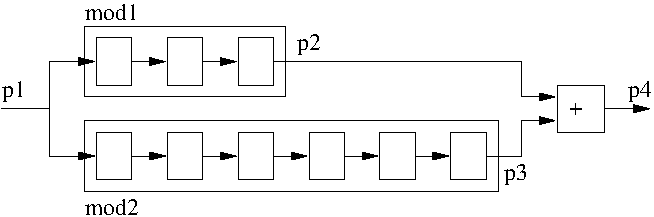
\includegraphics{pqueue}
        \caption{alternate pipeline paths}
        \label{fig:pqueue}
        \end{figure}
        Here the first shorter path will fill queue \var{q2} after 5 clock cycles (
        assuming \var{q1} is always available). The last statement cannot execute
        because \var{q3} is not yet available, the second pipeline path being longer.
        The buffer in q2 is now full so it becomes unavailable for writing and the same
        will apply through the first pipeline. But this means that the first pipeline
        will stop reading \var{q1} which means that the second branch has not yet
        reached the output but cannot continue to read \var{q1}. The data already in
        the second pipeline will continue to move through the queue but no more input to
        that queue will occur. When the data in the second pipeline reaches the output
        the last assignment statement can now execute until it exhausts the second
        pipeline. The two pipeline branches are interacting and this will slow
        throughput to about half. This interaction can be eliminated by making the queue
        buffer depth of queue \var{q2} large enough to keep accepting data until the
        second pipeline fills. The example would be fixed by -
        \begin{lstlisting}[language=threepl]
            queue({q1, q2, q3, p4}, "uint:8");
            attributes(q2, depth=16);

            mod1(q2 <- q1); // assume this module has 3 pipeline stages
            mod2(q3 <- q1); // assume this module has 6 pipeline stages
            p4 <<- q2 + q3;      
        \end{lstlisting}
        The buffer size is rounded up to various powers of two. Which powers of
        two, and the maximum allowed, depend on the FPGA - see the 3PL manual.




    \section{Target exceptions}

        3PL is designed for the generation of code which will process continuous
        data streams. If an exception condition arises it may prove necessary to
        prematurely exit from a conditional or loop block. In particular a
        statement within a block may be waiting for queue availability where
        the exception condition is such that this will not occur. A way is
        needed to force an exit from loops, code blocks or blocked statements.

        The following target constructs may have an {\bf unless} clause attached -
        \blist
        \item   {\bf seq \{\}}
        \item   {\bf par \{\}}
        \item   {\bf sync \{\}}
        \item   {\bf when ()}
        \item   {\bf when () else}
        \item   {\bf seq while () \{\}}
        \item   {\bf par while () \{\}}
        \item   {\bf sync while () \{\}}
        \item   {\bf seq do \{\} while ();}
        \item   {\bf par do \{\} while ();}
        \item   {\bf sync do \{\} while ();}
        \blend

        For example a seq block may have some queue reads which we want to terminate
        when an exception condition occurs -
        \begin{lstlisting}[language=threepl]
            static({s1, s2}, ...);
            queue({q1, q2}, ...);
            value(e, "log", ...);

            seq {
                s1 <- q1;
                s2 <- q2;
            } unless (e)
        \end{lstlisting}
        The {\bf seq} is at the top level and will execute in an infinite loop. If
        \var{e} is true the {\bf seq} will immediately terminate on the next clock
        edge. If any assignments in the {\bf seq} were ready to execute on that clock
        edge they will do so. Following termination the normal sequence of execution of
        the thread will continue, in this case the {\bf seq} immediately executing
        again. This is probably not what we want - there is usually some corrective
        code we wish to execute. To do this  there is an optional execution block
        associated with the {\bf unless}, e.g. -
        \begin{lstlisting}[language=threepl]
            static({s1, s2}, ...);
            queue({q1, q2}, ...);
            value(e, "log", ...);

            seq {
                s1 <- q1;
                s2 <- q2;
            } unless (e) {
                reset(q1, q2);
            }
        \end{lstlisting}
        The exception code body is in braces and may contain a number of statements,
        however it can only contain one target statement. That target statement
        may of course be a {\bf seq \{\}}, {\bf when ()},  {\bf par while () \{\}} etc.
        The exception code block is executed after the terminated block, following
        which normal thread execution will continue.

        Target statements with {\bf unless} clauses cannot be nested\footnote{Nesting
        of target statements with {\bf unless} clauses may be allowed in the future
        if and when I can figure out the complicated logic to do it.}.


    \section{combinatorial output memory}

        Combinatorial output memory can be used as a combinatorial function on read,
        i.e. when an address is present at the input the memory output will reflect
        the value stored at that address after a short delay. A memory read does not
        require a clock. A memory write is clocked. In the case of Xilinx FPGAs
        combinatorial output memory is distributed CLB RAM.

        Combinatorial output memory is accessed by means of variables whose mode
        is \kwd{cmemory}. These can only be created by the inbuilt procedure
        \kwd{cmemory()}, e.g.
        \begin{lstlisting}[language=threepl]
            int(ports, 2);
            str(dtype, "uint:8");
            str(atype, "uint:6");
            var(init, "[]uint", {.., .., .., .., ..    , ..});
            cmemory(m1, ports, atype, dtype, init);
        \end{lstlisting}
        The first argument to \kwd{cmemory()} is the identifier for the created
        variable. The second argument is the number of ports which for Xilinx
        can be 1 or 2. The address type and data type follow. These can be any type
        at all but the address type is restricted to a maximum width of 9 bits.
        The last argument is initialisation data for the memory and is optional.
        The initialisation argument is shown in the example as an array variable
        but it could be a list of values in braces. Where an array variable is
        used it could of course contain values computed in an immediate execution
        loop, e.g. values implementing a mathematical function or a translation table.

        If the memory has more than one port the ports can be accessed independently.
        In the case of Xilinx the second port, port 1, is read-only. The ports can
        be accessed at multiple places in the code but the code must be written
        to ensure that access on a port is mutually exclusive as access conflicts are
        not detected or resolved.

        Because the memory behaves as a combinatorial element on reading, the memory
        output is accessed via an inbuilt function, e.g.
        \begin{lstlisting}[language=threepl]
            static(d, dtype);
            static(a, atype);
            static(l, "log");

            when (l)
                d <- cmemoryread(m1, 0, a) + 3;
        \end{lstlisting}
        The memory data is available in the same clock cycle that the read occurs
        because it does not have to wait for a clock - the address propagates through
        the memory emerging as the stored data element at the output.

        This example uses static variables. When \var{l} is true \var{d} is
        assigned the sum of the memory output from port 0 at address \var{a} and
        the constant 3. We could also use queue variables, e.g.
        \pagebreak
        \begin{lstlisting}[language=threepl]
            float(gamma, 0.45);
            float(gain, pow(256.0, 1.0 - 1.0 / gamma));
            str(dtype, "uint:8");
            var(init, "[256]uint");
            for (int(i) ; i<256 ; i++)
                init[i] = round(gain * pow((float)i, 1.0 / gamma));
            cmemory(gamma_correct, 1, dtype, dtype, init);
            queue({q1, q2}, dtype);

            .
            .
            q2 <<- cmemoryread(gamma_correct, 0, q1);
            .
            .
        \end{lstlisting}
        where the memory read occurs whenever queues \var{q1} and \var{q2} are
        available (writing of \var{q1} and reading of \var{q2} are not shown in
        the code fragment). This example purports to show an 8-bit pixel gamma
        correction (I may have the function wrong, but you get the idea). The
        gamma correction lookup table is a cmemory mode variable with one port.
        The address input and data output are each 8 bits wide. The initialisation
        array has its contents computed during immediate execution using the
        value initially assigned to floating point variable \var{gamma}. The
        floating point values are rounded back to the nearest integer for
        assignment to the initialisation array\footnote{3PL provides
        target floating point format but arithmetic operations are logic-intensive and
        must be pipelined, i.e. FP operations cannot be done in one step in one
        clock cycle. There is a library of pipelined floating point operations.}.
        A variation is to use a two-port cmemory and allow table entries to be
        overwritten from an external CPU when required. The ZYNQ platform and
        various boards with a serial interface provide this facility and the
        above code might then be written as -
        \begin{lstlisting}[language=threepl]
            class(cpu, cpu_api());
            str(dtype, "uint:8");
            cmemory(gamma_correct, 2, dtype, dtype); // 2 ports, separate for read and write
            queue({wdata, waddr, q1, q2}, dtype);
            cpu.write_queue(wdata <- 1);
            cpu.write_queue(waddr<- 2);

            cmemorywrite(gamma_correct, 0, waddr, wdata);

            .
            .
            q2 <<- cmemoryread(gamma_correct, 1, q1);
            .
            .
        \end{lstlisting}
        The library module \kwd{cpu\_write\_queue()} allows a CPU coupled to the FPGA
        to write to a queue variable in the FPGA. The input arguments \var{1} and
        \var{2} are memory-mapped bus addresses for the bus interface to the FPGA.
        In this example the \kwd{cmemorywrite()} inbuilt procedure will write to the
        memory when queues \kwd{waddr} and \kwd{wdata} are both available.

        Of course we could combine a more complicated execution thread
        with queue variables -
        \pagebreak
        \begin{lstlisting}[language=threepl]
            struct(s,
                sum,    "uint:16",
                count,  "uint:16"
            );
            queue(dp, s);
            queue(ap, atype);
            static(count, "uint:16");
            static(accum, "uint:16");

            seq {
                sync while (ap != 0) {
                    accum <- accum + cmemoryread(m1, 0, ap);
                    count++;
                }
                sync {
                    dp.sum <<- accum;
                    dp.count <<- count;
                    count <- 0;
                    accum <- 0;
                }
            }
        \end{lstlisting}
        Here we loop reading memory and accumulating the sums of the values until
        the queued address is zero, at which point the sum and count are written
        to a queue (whose type is a struct containing fields for both values) and
        the static variables are cleared for the next iteration. The seq block then
        repeats.

        In this last example if the input queue \var{ap} transmits all zeros the
        output data stream \var{dp} will be at the same rate, otherwise the output
        will be at a lower rate which depends on the length of non-zero sequences.
        This is a characteristic of a systolic network with buffered queues, compared
        with a normal signal processing lock-step approach, that each datum can
        proceed through the network at a rate determined by producers and consumers
        at each node of the network. Where all inputs to the network have data available
        and each node can execute in one clock cycle then data can flow at clock rate.
        Where data input is sporadic or at sub-clock-rate, or multiple sequential
        execution cycles are needed at some nodes, the data throughput will be slower.




    \section{registered output memory}

        Registered output memory uses a clock for both read and write. On executing a
        read the data appears at the output following the next clock edge. In the case
        of Xilinx FPGAs registered output memory is block RAM.

        Because the memory output is delayed one clock cycle on a read, registered
        output memory reads must be pipelined, otherwise a read will take two clock
        cycles.

        Registered output memory is accessed by means of variables whose mode
        is \kwd{rmemory}. These can only be created by the inbuilt procedure
        \kwd{rmemory()}.

        In the previous section we had an example where data bytes were streamed
        through a look-up table for gamma correction -
        \begin{lstlisting}[language=threepl]
            type(dtype, "uint:8");
            cmemory(gamma_correct, 2, dtype, dtype);
            queue({wdata, waddr, q1, q2}, dtype);

            .
            .
            q2 <<- cmemoryread(gamma_correct, 1, q1);
            .
            .
        \end{lstlisting}
        We could convert that example to use registered output memory as follows -
        \begin{lstlisting}[language=threepl]
            type(dtype, "uint:8");
            rmemory(gamma_correct, 2, dtype, dtype);
            queue({wdata, waddr, q1, q2}, dtype);

            .
            .
            seq {
                rmemoryread(gamma_correct, 1, q1);
                q2 <<- rmemoryout(gamma_correct, 1);
            }
            .
            .
        \end{lstlisting}
        The seq loop will first attempt to execute a memory read from port 1 taking
        the address from queue \var{q1}. If \var{q1} is not available then the read
        will wait until it is. When the read has occurred the seq block will then
        execute the assignment of the current output value of the memory to queue
        \var{q2} (if \var{q2} is not available it will wait). The inbuilt function
        \kwd{rmemoryout()} gets the contents of the output register of the block RAM
        for the specified port. This value will remain in the output register until
        another memory read is executed. This code example does not pipeline the
        memory reads and hence takes two cycles per access.

        Note that in this example \kwd{rmemoryread()} is a procedure, not a module,
        so the module in which \var{q1} is being read is the file module.
        Since there is only one sink for queue \var{q1} we do not need to worry
        about ensuring that bits of the code are in separate modules and hence
        all the code is in the file module. If queue \var{q1} was also
        read by other unrelated code we would have to ensure that the reads were
        in separate modules so that the independent reads were handled correctly.

        To pipeline the above example the memory read must be separated from the
        following memory output value assignment. The assignment is dependent on
        a previous memory read so we need to signal that this has occurred. This
        could be done with another queue variable -
        \begin{lstlisting}[language=threepl]
            type(dtype, "uint:8");
            rmemory(gamma_correct, 2, dtype, dtype);
            queue({wdata, waddr, q1, q2}, dtype);
            queue(read, "log");

            .
            .
            sync {
                rmemoryread(gamma_correct, 1, q1);
                read <<- true;
            }

            when (read)
                q2 <<- rmemoryout(gamma_correct, 1);
            .
            .
        \end{lstlisting}
        but this code is not correct! If queue \var{q2} becomes unavailable for
        writing the assignment to it will wait but the next memory read may go
        ahead, overwriting the previous registered memory output value. We could
        acknowledge back via another queue but that would introduce an extra clock
        cycle.

        We need to execute the memory read and assign the result in the one clock.
        Since the read must occur in a clock cycle previous to the assignment to q2
        the two operations can be staggered by doing an initial read prior to
        entering the loop.
        \pagebreak
        \begin{lstlisting}[language=threepl]
            type(dtype, "uint:8");
            rmemory(gamma_correct, 2, dtype, dtype);
            queue({wdata, waddr, q1, q2}, dtype);

            .
            .
            seq {
                rmemoryread(gamma_correct, 1, q1);
                sync {
                    q2 <<- rmemoryout(gamma_correct, 1);
                    rmemoryread(gamma_correct, 1, q1);
                }
            }
            .
            .
        \end{lstlisting}
        here -
        \blist
        \item   the first statement in the {\bf seq} block executes the first read
        \item   the second statement in the {\bf seq} is an infinite loop
        \item   the loop sync block will not execute until {\bf q1} and {\bf q2} are
                available ({\bf q1} is not empty and {\bf q2} is not full)
        \item   {\bf q2} is assigned the previous result and the next read are performed
                simultaneously
        \item   the {\bf seq} block never completes
        \blend

        ANother approach is to create a module to handle pipelined
        rmemory reads -
        \begin{lstlisting}[language=threepl]
            type(dtype, "uint:8");
            rmemory(gamma_correct, 2, dtype, dtype);
            queue({wdata, waddr, q1, q2}, dtype);
            queue(read, "log");

            .
            .
            rread(q2 <- gamma_correct, 1, q1);
            .
            .
        \end{lstlisting}
        The code for the module might be -
        \begin{lstlisting}[language=threepl]
            global module
            rread (queue(data) <- rmemory(m), int(port), queue(addr)) {
                static(hold, "log");
                when (!hold || >data)
                    rmemoryread(m, port, addr);
                when (hold)
                    data <<- cast(rmemoryout(m, port), type(data));
                hold <- <addr || hold && !>data;
            }
        \end{lstlisting}
        We have declared the module as \kwd{global} so that it can be used anywhere -
        the scope of variables, modules, procedures and functions is discussed in
        a later section. In this module a static boolean variable \var{hold} is used
        to synchronise the memory reads and output queue assignments. When \var{hold}
        is true a value is held in the memory output register waiting to be assigned
        to the output queue. There are three statements in this module, each one
        executing independently in its own implicit infinite loop.

        The first statement executes a memory read if the hold flag is false (there
        is currently no unassigned registered memory output value) or if the output
        queue is available for writing (the {\bf \verb'>'} unary prefix operator returns
        true if the queue variable to which it is applied is available for writing -
        there is a similar operator, {\bf \verb'<'} for read availability). If
        {\bf \verb'<'}q1 is not true the statement will wait until it is true.

        The second statement assigns the registered memory output value to the output
        queue when \var{hold} is true. If the output queue \var{data} is not available
        this statement will wait untli it is available then execute the write.

        The third statement continually updates the value of \var{hold} - it is
        assigned true if an input is available or it is already true and the output
        queue is not available, otherwise it is assigned false.

        This module is already included in a 3PL library.


    \section{Clocks}

        A clock is another mode of variable - mode \kwd{clock}. A Clock variable can
        represent -
        \blist
        \item   a clock input from an input buffer driven from an FPGA pad
        \item   a clock signal between a digital clock manager and a global
                clock buffer
        \item   a clock signal distributed over a clock net driving FPGA
                synchronous logic 
        \blend

        A clock mode variable is created by calling the inbuilt procedure
        \kwd{clock()}. For an input clock signal various attributes such as
        the frequency and the FPGA pin(s) must be supplied. For example -
        \begin{lstlisting}[language=threepl]
            str(c100_pin, "E17");
            clock(c100, frequency=1.0e8, loc=c100_pin);
        \end{lstlisting}

        If the clock variable does not represent the output of an input clock buffer then
        there is no location attribute.

        If a clock is passed as an argument to a module, procedure or function
        then the parameter is not given any attributes, e.g.
        \begin{lstlisting}[language=threepl]
            procedure
            p (.... <- clock(c)) {
                .
                .
            }
        \end{lstlisting}

        To generate a clock a digital clock manager (DCM) is used. The following code
        illustrates this -
        \begin{lstlisting}[language=threepl]
            str(c100_pin, "E17");
            clock(c100_in, frequency=100.0, loc=c100_pin, ibufg=true);
            clock({global.c100, c100_raw});
            clkdcm(clk0=c100_raw <- clkin=c100_in, clkfb=c100);
            clockbuffer(c100 <- c100_raw);
        \end{lstlisting}
        \begin{figure}[htbp]
        \centering
        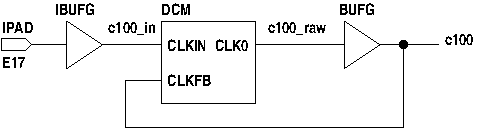
\includegraphics{dcm}
        \caption{digital clock manager}
        \label{fig:dcm}
        \end{figure}
        Creating c100 with global scope ensures that it is globally accessible
        where \kwd{c100\_in} and \kwd{c100\_raw} may have local scope.
        Library procedures \kwd{clkdcm} and \kwd{clockbuffer} both propagate
        the frequency and period attributes from inputs to outputs so we don't
        have to assign these attributes to \kwd{c100\_in} and \kwd{c100\_raw}.

        Before any logic involving synchronous elements is generated by 3PL the
        clock domain must be established. This is done by calling the inbuilt
        procedure \kwd{useclock()}, e.g.
        \begin{lstlisting}[language=threepl]
            useclock(c100);
        \end{lstlisting}

        When the clock domain is changed using \kwd{useclock()} the previous clock domain
        is pushed onto a stack. If \kwd{useclock()} is called with no argument the previous
        clock domain is popped off the stack and again becomes the current clock domain.

        The clock domain used by variables is established when they are assigned
        or evaluated, not when they are created.

        For a static variable the clock domain in use when the variable is assigned
        a value or is evaluated establishes the clock domain for the variable. Any
        other assignments or evaluations of that variable must be in the same clock
        domain.

        For a queue variable the read and write clock domains may be different. The write
        clock domain is established by the clock domain in use when the first write is
        encountered and all subsequent writes must be in the same clock domain. Similarly
        the read clock domain is established by the clock domain in use on the first read
        of the queue and all subsequent reads must be in the same clock domain. If the read
        and write clock domains are the same, which is the usual case, the queue is called
        {\bf synchronous} and the queue buffer depth will be 2 by default. If the read and
        write clock domains differ the queue is called {\bf asynchronous} and the default
        buffer depth is 16. Resynchronisation of queue data between the two clock domains
        is handled automatically by the asynchronous queue.

        In general in a statement the clock domain in use must agree with the clock
        domain of variables that are assigned or evaluated in that statement.
        Procedure and module calls are an exception in that the clock domains are
        checked in the body of the called module or procedure but not when arguments
        are evaluated and passed to parameters.

        The correct way to pass data from one clock domain to another is via an
        asynchronous queue, however there are two functions, \kwd{accept()} and
        \kwd{sample()} which allow mixing of clock domains at the programmer's
        peril. \kwd{accept()} simply overrides the clock checks and can be used if
        data is seldom changed and the risk of data corruption is acceptable (safe
        for single bit data except for the very small probability of getting a
        metastable state. For single bits an inbuilt function \kwd{resync()} can be
        used to do this properly). \kwd{sample()} preserves data integrity by
        resampling it into the current clock domain, however since the clock
        frequencies differ a datum may be lost or duplicated (but will not be
        corrupted).


    \section{Modules}

        Modules and procedures were briefly mentioned in the context of queue variables. A
        module has the important property that it delineates a sink for queue variables.
        When a Queue has more than one sink each sink must execute a read on the queue
        before the datum is popped and the next becomes available. Multiple reads within a
        sink are treated as a single read if they occur simultaneously, otherwise they are
        separate reads. A queue has two sinks if the two code sections which read the queue
        are in different modules, For example -
        \begin{lstlisting}[language=threepl]
        queue({p, q1, q2}, t1);

        .
        p <<- .....;
        m1(q1 <- p);
        m2(q2 <- p);
        .

        module
        m1 (queue(pout) <- queue(pin)) {
            pout <<- p - 3;
        }

        module
        m1 (queue(pout) <- queue(pin)) {
            pout <<- p * 2;
        }
        \end{lstlisting}
        Modules are declared with output parameters followed by input parameters,
        these lists being separated by {\bf \verb'<-'} (the left arrow can be
        omitted if there are no output parameters). Each parameter is a call to
        an inbuilt variable creation procedure. References to parameters in
        the module code body are replaced by the arguments passed in the call.
        If a parameter is not passed an argument then it becomes a local variable.
        For this reason parameters can have initial values which become the
        variable initial values if no matching argument is provided. There is
        an inbuilt procedure {\bf matched()} which can be used to test if a
        parameter has been passed an argument. Arguments are normally matched
        to parameters by the order in which both occur however an alternative
        is to use {\bf parameter=argument} pairs in the call. This is useful
        where there are many parameters and only a few are to be passed arguments.
        A combination of both modes is allowed as long as no positional arguments
        follow any parameter=argument pairs.

        Parameters can have target type widths missing, dimensions missing or
        even a type missing or a mode missing. The missing elements will be filled
        in from the argument. Where parameters have types and dimensions these
        will be checked against the argument type and dimensions. An exception
        is target numeric type widths which allow a mis-match, resulting in truncation
        or padding.

        A module is a block of code which can be called. Module calls are
        only done during immediate execution. There is no code in the FPGA which
        executes any sort of shared code call! When a module is called however
        any target statements that it contains are established as independent
        execution streams. A module call would not usually be made within a target
        construct such as a \var{when} or one of the target loops. In contrast
        a procedure containing a target statement called within a target construct
        will result in that statement appearing in-line where the call is made.

        Declaring a module and calling it can be verbose and inconvenient, especially if
        the code blocks are small and the modules are only called once. Instead an un-named
        module can be used. An un-named module is code enclosed in square brackets. It is
        not called as such but simply appears in-line, though it is executed as a distinct
        and separate module from that within which it is nested. The above code could be
        written
        \begin{lstlisting}[language=threepl]
        queue({p, q1, q2}, t1);

        .
        p <<- .....;
        [q1 <<- p - 3;]
        [q2 <<- p * 2;]
        .
        \end{lstlisting}
        where now the assignments to queues \var{q1} and \var{q2} are in separate
        modules - the code in brackets. Un-named modules do not have calls and hence
        there are no arguments and parameters. The scope of an un-named module is like
        that of a code block in braces. Variables created inside the brackets are in
        the scope of the un-named module. But code within the un-named module can
        access the scope in which it is enclosed - in the case above \var{p}, \var{q1}
        and \var{q2} occur in the scope outside the two un-named modules but are
        accessible within the un-named modules.

        Note that in this example the assignment to \var{q1} will occur when both
        \var{q1} and \var{p} are available. Similarly  the assignment to \var{q2} will
        occur when both \var{q2} and \var{p} are available. If \var{q1} and \var{q2}
        become available at different times the assignments will not occur
        simultaneously, but each will read the same datum from \var{p} since \var{p}
        will not pop its datum until both reads have occurred (the first read to occur
        will not see \var{p} become available again until after the second read has
        occurred). If instead the code was
        \begin{lstlisting}[language=threepl]
        queue({p, q1, q2}, t1);

        .
        p <<- .....;
        q1 <<- p - 3;
        q2 <<- p * 2;
        .
        \end{lstlisting}
        it would function correctly if all three queues were available, both \var{q1}
        and \var{q2} being assigned the datum from \var{p}. If however \var{p} and
        \var{q1} were available but \var{q2} was not, the assignment to \var{q1} would
        take place and the datum would be popped from \var{p}. When \var{q2} became
        available it would read the next datum from \var{p}. Another solution might be 
        \begin{lstlisting}[language=threepl]
        queue({p, q1, q2}, t1);

        .
        p <<- .....;
        sync {
            q1 <<- p - 3);
            q2 <<- p * 2);
        }
        .
        \end{lstlisting}
        which inhibits both assignments until all three queues are available.



    \section{Modules, procedures, functions and classes}

        3PL provides user-defined procedures and functions.

        Briefly -
        \blist
        \item   module, procedure, function and class calls are only executed during
                immediate execution - the calls are not executed in the FPGA
        \item   modules and procedures are called using the same syntax and semantics
        \item   modules and procedures are declared the same way except for the
                keyword {\bf module} or {\bf procedure}
        \item   a module may contain any number of target statements whereas a
                procedure can contain at most a single target statement (but which
                may be a seq, par sync etc.)
        \item   each target statement in a module is established in its own
                execution thread whereas the single target statement in a procedure
                is executed in-line at the location of the call
        \item   modules and procedures with no target statements are functionally
                identical
        \item   modules delineate queue sinks but procedures do not
        \item   functions can only appear within the context of an expression -
                they cannot be called using module or procedure call syntax
        \item   functions can return immediate or target values
        \item   functions cannot contain in-line target statements - they can
                contain module calls
        \item   classes are called in a similar manner to modules or procedures but
                they return a value, a class instance
        \item   a class cannot contain in-line target statements
        \blend

        A procedure call and definition are illustrated by the following example -
        \begin{lstlisting}[language=threepl]
            static(s, "uint:8");    // unsigned integer of 8 bits
            static(v, "[2]uint:8"); // array of 2 unsigned integers of 8 bits

            p(s <- v[0], v[1] + 2, 3);

            procedure
            p (static(os, "int:8") <- value({iv1, iv2}, "int:8"), int(i)) {
                os <- iv1 + (iv2 >> i);
            }
        \end{lstlisting}
        This procedure, \var{p}, has one output parameter, the 8-bit integer
        static mode variable \var{os}, and three input parameters, two
        value variables and an immediate integer variable. Parameters are created
        by using the same variable creation procedures as before.

        procedures have their own variable scope so any variables created in the
        body of the procedure (and any unmatched parameters) are in the local
        scope of the procedure and cannot be accessed from outside the procedure,
        including any deeper calls to procedures (or functions).

        The convention for both procedure definitions and calls is that parameter and
        argument lists consist of outputs, \verb'<-' and then inputs. If there are no
        output parameters in the definition the \verb'<-' can be omitted. Similarly if
        there are no output arguments in the call the \verb'<-' can be omitted. For
        value and immediate mode input parameters the argument is copied to the
        parameter by assignment, i.e. it is call-by-value. For other input parameter
        modes and for all output parameters the parameter 'points' indirectly to the
        argument variable, i.e. call-by reference.

        A value mode input parameter can be passed an argument which is an expression,
        and that expression could be immediate mode (i.e. a constant in the target).
        Similarly an immediate mode input parameter can be passed an argument which
        is an expression, however that expression must be immediate mode, not a
        target mode. In the example above the first input parameter is value mode
        and has been passed one member of a static mode array. The second value
        mode parameter has been passed an expression which is the sum of a
        member of a static mode array and a constant. The body of the procedure
        adds the first parameter to the second parameter right shifted by the
        third and assigns the result to the output static variable.

        For the other cases these are call-by-reference and any reference to the
        parameter accesses the actual variable passed as an argument. Note that
        where the type is an array the argument may be a sub-array,
        e.g. -
        \begin{lstlisting}[language=threepl]
            static(v, "[6]uint:8");

            p(v[1..3]);

            procedure
            p (static(p, "[3]int:8")) {
                ...
            }
        \end{lstlisting}
        This applies to call-by-value and call-by -reference and to both input and
        output parameters.

        If parameter dimensions are given the argument dimensions must be the same,
        however we could omit the parameter dimensions to make the procedure more
        flexible -
        \begin{lstlisting}[language=threepl]
            static(v, "[6]uint:8");

            p(v[1..3]);

            procedure
            p (static(p, "[]int:8")) {
                println(dimensions(p));     // print the number of dimensions of p
                println(dimension(p, 0));   // print the first dimension of p
            }
        \end{lstlisting}
        which would print
        \begin{lstlisting}[language=threepl]
            1
            3
        \end{lstlisting}

        Arguments may be omitted in which case the unmatched parameters become
        local variables in the procedure. Input parameters may be given initial values
        so that these values will be used if no matching argument is passed.

        Arguments are assigned to parameters in left to right order with inputs
        assigned before outputs. This means that when a parameter is created
        the type argument to the inbuilt variable creation procedure could use
        values passed to parameters to the left.

        A parameter can be tested to determine if an argument has been passed to it by
        means of the inbuilt function \kwd{matched()} which returns true if an argument
        has been passed.

        In addition to the usual matching of arguments to parameters by position
        the keymatch format may be used where each argument is identifier=value,
        the identifier being that of the parameter. The keymatch arguments can be
        in any order but arguments are assigned to parameters in parameter order.
        Positional arguments can precede keymatch arguments but cannot follow them.

        Considerable flexibility is allowed in argument passing. Missing parameter
        dimensions can be inferred from the argument dimensions and target type widths
        need not be the same (truncation or padding will result if not).

        Procedures may contain immediate statements however they may only contain at
        most a single in-line\footnote{This qualification will be explained later.}
        target statement! This statement may be a control structure containing other
        target statements nested to any depth. The following procedure definition -
        \pagebreak
        \begin{lstlisting}[language=threepl]
            procedure
            p () {
                a <- 3; //
                b <- 4; // ILLEGAL!
            }
        \end{lstlisting}
        is not allowed. It is not clear what is to be done with two target statements.
        If \var{p()} is called at the top level you might expect the assignments to be
        placed in their own infinite loops. If called in a par{} or seq{} block then
        perhaps they are added to the block. To avoid this uncertainty procedures
        can only contain one target statement but of course this can be a
        \kwd{par\{\}}, \kwd{seq\{\}}, \kwd{when}, \kwd{seq while}, \kwd{par while} etc.

        Functions differ from procedures in that -
        \blist
        \item   there are no output parameters
        \item   there are no in-line target statements
        \item   a function call appears where a value is required, not on
                a line by itself as for a procedure call.
        \item   there is a return statement to return a value - this can only
                be immediate mode or value mode
        \blend

        Functions have local variable scope in the same way as procedures.

        Functions cannot have target statements but they can have target
        expressions and return values. The following illustrates a trivial
        function returning a target mode value -
        \begin{lstlisting}[language=threepl]
            function
            add (value({a, b}, "int:8")) {
                value(v, "int:9")
                v := a + b;
                return(v);
            }
        \end{lstlisting}
        Note that the declaration does not define the return type, so a function
        could have several different return types governed by conditional
        statements.

        The trivial example above is verbose and could be recoded as -
        \begin{lstlisting}[language=threepl]
            function
            add (value({a, b}, "int:8")) {
                value(v, "int:9", a + b)
                return(v);
            }
        \end{lstlisting}
        or simply -
        \begin{lstlisting}[language=threepl]
            function
            add (value({a, b}, "int:8")) {
                return(a + b);
            }
        \end{lstlisting}

        It was previously stated that procedures could contain at most one in-line
        target statement and functions could not contain any. The term "in-line"
        excludes statements contained in modules within a procedure or functions. The
        reason is that a module is an independent block of code that originates target
        execution threads. If a procedure contains a target statement that statement is
        in-line, i.e. that statement will be inserted into the target execution thread
        in the context where the procedure is called. When a module is called it
        establishes a completely new context for establishing execution threads
        unrelated to the context in which it is called. As an example suppose we wish
        to write a function which returns a value which is the value of the argument
        delayed by a number of clock cycles. The function cannot contain target
        statements so it seems that we could not write this, but a function can contain
        a module which in turn can contain target statements. We could write the
        function as follows -
        \pagebreak
        \begin{lstlisting}[language=threepl]
        global function
        del (value(in), int(n, 1)) {
            type(t, type(in));
            static(d, "["+n+"]t");

            [
                d[0] <- in;
                for (int(i, 1) ; i<n ; i++) // loop for i from 1 to n-1
                    d[i] <- d[i-1];
            ]

            return(d[n-1]);
        }
        \end{lstlisting}
        The first input parameter has no type specified so it will use the type of its
        argument. The second argument is immediate and is the delay count. It is set to
        default to 1 if it is not given an argument. Note that the array type is
        constructed as a string expression to insert the dimension gained from the
        second parameter. The value returned for the function is value mode and is the
        value of the last member of the static variable array. Note that the loop
        starts at index 1 as the loop variable \var{i} is initialised to 1.

        The un-named module can access the scope of the function in which it is
        contained. Note that the assignments to variable \var{d} are not in a par
        block. Since we are at the top level of a module each assignment statement will
        execute in parallel in its own infinite loop at clock rate\footnote{The code
        generator will eliminate the loop and simply control the enables to the
        register flip-flops. How and when these are asserted depends on how execution
        in the FPGA is started. It can be started by an external signal or it can start
        spontaneously after configuration - see target-execution-start in the manual
        index. A static variable can have its 'continuous' attribute set to true in
        which case the enables will be tied high.}.

        Procedure and function calls can be recursive. This is a very powerful
        mechanism allowing very simple and concise code to be written. Recursion
        often offers solutions that cannot be written iteratively. Any target code
        is duplicated on each call.

        We could instead write the above example recursively -    
        \begin{lstlisting}[language=threepl]
        global function
        del (value(in), int(n, 1)) {
            if (n == 0)
                return(in);
            static(d, type(in));
            [d <- in;]
            return(del(d, n-1));
        }
        \end{lstlisting}
        Each call to the function delays zero or one clock cycles. If the count
        is non-zero it delays the input by one cycle then calls itself with the
        result and a count minus 1. The assignment again is within an un-named
        module but now it is a single statement. There will be {\em n}
        un-named modules created, each with one assignment.

        When writing iterative code note that it can be convenient to
        use a value variable which is re-assigned on every iteration. The following
        function ORs the bits of its argument.
        \begin{lstlisting}[language=threepl]
        global function
        orbits (value(v, "bits:")) {
            int(n, dimension(v));
            value(ret, "log", cast(getbit(v, 0), "log"));
            for (int(i, 1) ; i<n ; i++)
                ret := ret || cast(getbit(v, i), "log")
            return(ret);
        }
        \end{lstlisting}
        The value variable \var{ret} is initially the LSB of the input but each time
        around the loop it is re-assigned the OR of itself and the next successive bit
        from the input. Finally it is returned as the value of the function. Note that
        the function parameter has no data width - this is derived from the
        argument. We could make two changes to this example. First we could generalise
        it so that it would accept any type for the input. Secondly we could
        avoid the use of the library function \var{getbit()} by casting the input
        into an array of "log".
        \begin{lstlisting}[language=threepl]
        global function
        orbits (value(v)) {
            int(n, size(v));
            value(vx,, forcecast(v, "["+n+"]log"));
            value(ret, "log", vx[0]);
            for (int(i, 1) ; i<n ; i++)
                ret := ret || vx[i]
            return(ret);
        }
        \end{lstlisting}
        The library function \var{forcecast()} is a more extreme version of inbuilt
        function \var{cast()}.
        Where a value variable is given an initial value the type argument can be
        omitted since the type can be inferred from the initial value.

        Module, procedure, function and class definitions may be nested, so a function or
        procedure may be defined within another function or procedure and hence can
        only be called by the parent function or procedure. By this means the scope and
        hence accessibility of functions and procedures can be limited and procedure
        and function identifiers can be re-used locally without ambiguity.

        It may be apparent by now that modules, procedures, functions and classes are only
        called during immediate execution - they are not called within target code. There
        is no equivalent to a procedure or function call in the FPGA code. Indeed this
        would not make sense as it implies shared code and sequential access which defeats
        the purpose of using an FPGA for parallel execution. Procedures and functions are
        useful where the same code is needed multiple times, be it immediate code or target
        code, however the procedure and function calls only take place during immediate
        execution.

        Module, procedures, functions and classes accept a "varargs" parameter which will
        match any number of arguments of any type or mode. This must follow normal
        parameters if used.




    \section{program structure and scope}

        There are a number of variable scopes -

        \blist
        \item   global scope
        \item   file scope
        \item   local scope
        \item   block scope
        \blend

        Global scope is accessible anywhere. Variables are created in global scope if
        the variable identifier has "global." prepended when the variable creation
        inbuilt procedure is called. If the same variable identifier is used in more
        than one scope the global version can be explicitly selected by prepending
        "global.". Variables are never placed in global scope by default.

        When the 3PL compiler begins to compile source code from the source file passed
        to it on the command line it creates a module to contain that code. That module
        is called a {\bf file} module. A file module does not have an identifier since
        it is not explicitly called. Source code within that source file forms the code
        body of the file module and this is executed by the interpreter following
        compilation. Variables created immediately within the file module (i.e. not
        within nested blocks) by default are contained in the file module scope.
        If variables are created within code blocks nested within that file
        scope but their scope is required to be the file scope then their
        identifiers must have "file." prepended. Similarly if necessary a variable
        reference can be disambiguated by prepending "file.".

        3PL allows other source files to be nested within the command line source
        file. There are two mechanisms for doing that.

        A source file can be nested within another by the construction    
        \begin{lstlisting}[language=threepl]
            source "file.3pl"
        \end{lstlisting}
        This simply inserts the text of the file at that point in the current file.
        This can be done to any depth.
        This is equivalent to \#include in C. If instead the code
        \begin{lstlisting}[language=threepl]
            module "file.3pl"
        \end{lstlisting}
        is used the file is inserted as before however a new file module is created
        for which the new source file supplies the code body. again this can be done to
        any depth.

        Any variables created immediately within the new file module are by default
        contained in the file scope for that module. Again this can be made explicit
        by prepending "file." to the variable identifier.

        File scope is useful for hiding variables away from application code without
        the need to call a module for initialisation. For example a hardware
        interface is usually coded as a file module. The source file for this might be
        "gadget.3pl". By including this using the statement
        \begin{lstlisting}[language=threepl]
            module "gadget.3pl"
        \end{lstlisting}
        a file module will be created. Top level code within this file module will
        be interpreted at the point at which occurs in the enclosing source. This
        code will create variable, such as inputs, outputs, FPGA pin names etc. and 
        by default these will be in the file module scope. The module will also
        define modules, procedures and functions which provide the interface to the
        gadget. These can access the variables in file scope but the callers to
        these cannot access the variables. Hiding variables in this way both
        protects the interface from incorrect usage and also avoids accidental
        conflicts with variable identifiers.

        Within a module other than a file module, a procedure or a function variables
        created outside of nested code blocks are by default local to the module,
        procedure or function. They can be accessed anywhere within the module,
        procedure or function but not from any nested calls or from anywhere else.

        Within a code block in braces any created variables are in the scope
        of the block. A problem arises where variables are created conditionally.
        The code
        \begin{lstlisting}[language=threepl]
        procedure
        p (log(l)) {
            if (l)
                int(i);
        }
        \end{lstlisting}
        does what one would expect - creates the integer \var{i} in the scope
        of the enclosing procedure. If this is changed to
        \begin{lstlisting}[language=threepl]
        procedure
        p (log(l)) {
            if (l) {
                int(i);
                float(f);
            }
        }
        \end{lstlisting}
        two variables are created, but they are in the scope of the {\bf if} code
        block in braces, not in the scope of the procedure. To fix this the code
        should be changed to
        procedure
        p (log(l)) {
            if (l) {
                int(local.i);
                float(local.f);
            }
        }
        which creates the variables in the procedure scope.

        Suppose one wishes to write a procedure which creates variables. The code
        \begin{lstlisting}[language=threepl]
        procedure
        myvar (str(name), log(signed)) {
            if (signed)
                static(name->, "int:8");
            else
                static(name->, "uint:8");
        }
        \end{lstlisting}
        will create a variable whose identifier is derived from the string argument
        by using the indirect operator. The problem is that the variable is
        created in the local scope of the procedure, not the scope in which it is
        called. To achieve the latter it can be changed to
        \begin{lstlisting}[language=threepl]
        procedure
        myvar (str(name), log(signed)) {
            str(n, "calling." + name);
            if (signed)
                static(n->, "int:8");
            else
                static(n->, "uint:8");
        }
        \end{lstlisting}
        or more simply
        \begin{lstlisting}[language=threepl]
        procedure
        myvar (str(name), log(signed)) {
            if (signed)
                static(("calling." + name)->, "int:8");
            else
                static(("calling." + name)->, "uint:8");
        }
        \end{lstlisting}
        or even more simply
        \begin{lstlisting}[language=threepl]
        procedure
        myvar (str(name), log(signed)) {
            static(("calling." + name)->, signed ? "int:8" : "uint:8");
        }
        \end{lstlisting}

        When the interpreter encounters a reference to a variable it first searches
        the current code block, then back out through nested code blocks until it
        reaches the local scope of the enclosing module, procedure or function. This
        behaviour is the same  as exhibited by other common programming languages such
        as C or Java. If the variable has not been found the interpreter looks in the
        file (module) scope. Finally it looks in the global scope. If the variable
        identifier has "global.", "file.", "calling." or "local" prepended the
        interpreter explicitly expects to find the variable in the named scope.        

        When a non-inbuilt module, procedure or function is called, the interpreter
        searches from the current local scope back through the scopes of nested module,
        procedure and function {\bf declarations} (NOT calls) until it finds a match.
        If that fails it looks in global scope. Thus, like variables, module, procedure
        and function identifiers can be used in different scopes as long as there is no
        conflict. A module, procedure or function definition occupies the scope of the
        module, procedure or function in which it is defined unless the keyword
        \kwd{global} precedes the \kwd{module}, \kwd{procedure} or \kwd{function}
        keyword, in which case it has global scope, i.e. it can be called from anywhere.

        Nested declarations allow modules, procedures and functions to be limited
        in scope so that they can only be called locally. This also allows
        module, procedure and function identifiers to be re-used locally.





    \section{Selectvalue mode}

        Selectvalue mode creates busses using three-state buffers. A selectvalue
        variable can have a number of conditional assignments. The following is an
        example using this mode -
        \pagebreak
        \begin{lstlisting}[language=threepl]
        selectvalue(bus, "bits:8");
        value(address, "uint:4");
        value(write, "log");
        static(data1, "int:5");
        static(data2, "uint:7");

        when ((address == 3) && write)
            bus |- cast(data1, type(bus));
        when ((address == 7) && write)
            bus |- cast(data2, type(bus));
        \end{lstlisting}
        The assignment operator for a selectvalue is \verb'|-' which is intended
        to look a little like a diagram of a connection to a bus. A conditional
        assignment to an output mode variable uses the same assignment operator
        because again a three-state drive is involved.
        When variable \var{address} is 3 and \var{write} is true, drive \var{data1}
        onto \var{bus}.
        When variable \var{address} is 7 and \var{write} is true, drive \var{data2}
        onto \var{bus}.
        The value of variable \var{bus} can be used in expressions
        the same way as other modes such as value or static.
        It is often the case that a bus must be shared by data of different types.
        This example illustrates this. The bus type has been made {\bf bits} and
        variables \var{data1} and \var{data2} have been cast to that type. In both
        cases the variables have fewer bits than \var{bus} so \var{data2} will be
        zero padded to 8 bits and \var{data1} will be sign extended to 8 bits.



    \section{Priority mode}

        Priority mode creates a priority encoder. The type must be "[]log" where the
        array dimension is at least as large as the number of inputs (it may be larger
        and will be trimmed). The encoder is combinatorial and has the same number of
        outputs as inputs (or one extra, see below). If one or more inputs is true the
        output corresponding to the lowest subscript input which is true will be true,
        all other outputs being false. The following example arbitrates between two
        queue variables which are to be written to a common bus -
        \begin{lstlisting}[language=threepl]
        selectvalue(bus, "uint:8"); // bus
        priority(arb, "[10]log");   // bus arbitration variable
        queue({q1, q2}, "uint:8");   // bus sources

        arb[0] := <q1; // q1 is available for reading
        arb[1] := <q2; // q2 is available for reading

        when (arb[0])
            bus |- q1;
        when (arb[1])
            bus |- q2;
        \end{lstlisting}
        Since the lowest subscript applies to \var{q1} it will have priority
        over \var{q2} if both are available simultaneously. The priority
        variable is dimensioned 10 however the unused higher entries will be
        ignored. One additional output may be used, i.e. \var{arb[2]} in the case of
        the example. This extra output is true if none of the inputs is true.


    \pagebreak
    \section{More on types}

        Target variable types are -

        \begin{tabular}{| l | l |}
        \hline
        bits:{\em n}           & unspecified binary                 \\ \hline
        uint:{\em n}           & unsigned integer                   \\ \hline
        int:{\em n}            & signed integer                     \\ \hline
        log                    & logical                            \\ \hline
        fixed:{\em m} .{\em n} & fixed point                        \\ \hline
        float:{\em m} e{\em n} & floating point                     \\ \hline
                               & enumerated type                    \\ \hline
        null                   & no data                            \\ \hline
        \end{tabular}

        Immediate types are -

        \begin{tabular}{| l | l |}
        \hline
        bits      & unspecified binary                              \\ \hline
        uint      & unsigned integer                                \\ \hline
        int       & signed integer                                  \\ \hline
        log       & logical                                         \\ \hline
        str       & string                                          \\ \hline
        float     & floating point                                  \\ \hline
        \verb'->' & pointer                                         \\ \hline
        type      & type                                            \\ \hline
        list      & a list                                          \\ \hline
        map       & a map                                           \\ \hline
        file      & a file                                          \\ \hline
        empty     & take the type from an initialisation argument   \\ \hline
        \end{tabular}

        In both target and immediate modes the types can be nested within
        arrays or structs. Immediate and target mode types cannot be mixed
        within a struct.


    \section{Inbuilt modules, procedures and functions}

        We have already seen the use of inbuilt procedures such as \var{static()}
        and \var{queue()}. There are very many such inbuilt procedures, even more
        inbuilt functions and a few inbuilt modules. The inbuilt functions include
        the usual numeric and string operations which are for immediate execution only.



    \section{Libraries}

        3PL libraries are source code files that are incorporated into the source
        stream by {\bf source "..."} or {\bf module "..."} statements. It is usual to
        incorporate a library called a {\em header file} as the first line of source
        code. This header file is specific to the FPGA platform and sets up FPGA
        package pins definitions and clock logic and provides interfaces to
        external devices on the platform. There are other libraries which are more
        general and contain useful modules, procedures and functions. Often these
        are already incorporated in the header file.



    \section{Petri nets}

        State machines are a convenient way of expressing a control algorithm. When
        implementing state machines in FPGAs it is usual to represent each state
        by a flip-flop state\footnote{The alternative is to represent the state
        by a counter, which is the usual way in software.}. Exactly one state
        flip-flop should be set at any time. A state transition requires the
        current state flip-flop to be reset and another state flip-flop to be
        simultaneously set. A Petri net is a similar but more general scheme.
        The form of Petri net implemented in 3PL would be described as "a finite
        capacity Petri net with a capacity of 1" which is a less general form.
        Although it is a contradiction in terms one can think of this form of
        Petri net as a state machine implementation where more than one state
        flip-flop can be set at a time. Transitions can then involve some
        flip-flops being cleared and others set. A simple state machine can
        be described by a Petri net.

        In a Petri net we have {\em places} rather than {\em states} and each place
        can have a token (set) or no token (cleared). A transition involves taking
        tokens from one or more places and inserting them in one or more other places.
        Expressions describing when transitions are to take place are called
        {\em predicates}.

        The following is an example of the syntax -
        \begin{lstlisting}[language=threepl]
            petrinet {
                initial q1, q2;
                q1, q2 -> q3, p4 when (a && (b != 0)) {s <- queue1;};
                q3 ->> q1 {l1 <- queue1;};
                q4 -> q2, q3 when (!l2);
            }
        \end{lstlisting}
        Here there are places \var{q1}, \var{q2}, \var{q3} and \var{p4}. Each of these
        is a static variable of type "log". If they have not already been created the
        Petri net construct creates them. These variables cannot be assigned by any
        code, only by the Petri net mechanism itself, however their values can be used
        in the program code outside of the Petri net in the same way that ordinary
        variables are used.

        In the example places \var{q1} and \var{q2} initially have tokens. When the
        expression $a \&\& (b != 0)$ (called the {\em predicate}) is true and \var{q1}
        and \var{q2} both contain tokens (are set), \var{q1} and \var{q2} will have
        their tokens removed (are cleared) and places \var{q3} and \var{p4} have tokens
        inserted (are set). The single right arrow indicates a weak transition, meaning
        that prior to the transition any tokens in the destination places are ignored.
        If a double right arrow is used this signifies a strong transition, meaning
        that the transition can only occur if the destination places do not have
        tokens.

        In the example above the code block to the right of the first transition is
        executed when the transition occurs. It may contain
        only a single target statement (which can of course be a compound statement
        such as  {\bf seq\{\}}, {\bf par\{\}} etc.). If a transition does not have a
        predicate then it occurs when the source places have tokens (and optionally
        destination places lack tokens). A transition code block may contain immediate
        statements but these would serve little purpose as they are only executed as the
        interpretter passes through the code during immediate execution.

        To code a state machine as a Petri net the following apply -
        \blist
        \item   each transition has only one source and one destination place
        \item   only one place is initialised
        \item   transitions can be weak (it doesn't matter which are used, but
                weak transitions use fewer logic resources)
        \blend

